\section{Preliminaries}\label{sec:prel}

\subsection{Multisignatures}\label{sec:multisig}

A multisignature scheme~\cite{itakura1983public,CCS:MicOhtRey01} is a
tuple of algorithms:
$$
\ms = (\msSetup \times \allowbreak\msKeyGen \times \allowbreak\msCombVK \times \allowbreak
\msSign \times \allowbreak\msComb \times \allowbreak\msVfy)
$$
Where $\msSetup$ generates public parameters $\msParams$, such that
\begin{itemize}
  \item $(\msVK,\msSK) \gets \msKeyGen(\msParams)$ can be used to generate fresh key pairs,
  \item $\msSig \gets \msSign(\msParams,\msSK,\msMsg)$ signs  a message $\msMsg$ using key $\msSK$;
  \item $\msCSig \gets \msComb(\msParams,\msMsg,\msVKL,\msSigL)$ aggregates a
    set $\msSigL$ of signatures into a single, aggregate signature~$\msCSig$.
  \item $\msCVK \gets \msCombVK(\msParams,\msVKL)$ aggregates
  a tuple $\msVKL$ of verification keys $\msVK$ into a single,
  aggregate verification key $\msCVK$.
\end{itemize}
  $\msCVK$ can be used for verification:
  $\msVfy(\msParams,\msCVK,\msMsg,\msCSig) \in \{\true,\false\}$
  verifies an aggregate signature under an aggregate verification key.
  In the following, we often make the parameter~$\msParams$ implicit in the
    function calls for better readability.

  Intuitively, the security of a multisignature scheme guarantees
  that, if $\msCVK$ is produced from a tuple of verification keys
  $\msVKL$ via $\msCombVK$, then no aggregate signature $\msCSig$ can
  pass verification $\msVfy(\msCVK,\msMsg,\msCSig)$ unless all
  honest parties holding keys in $\msVKL$ signed $m$.

\begin{figure}[t]
  \centering
 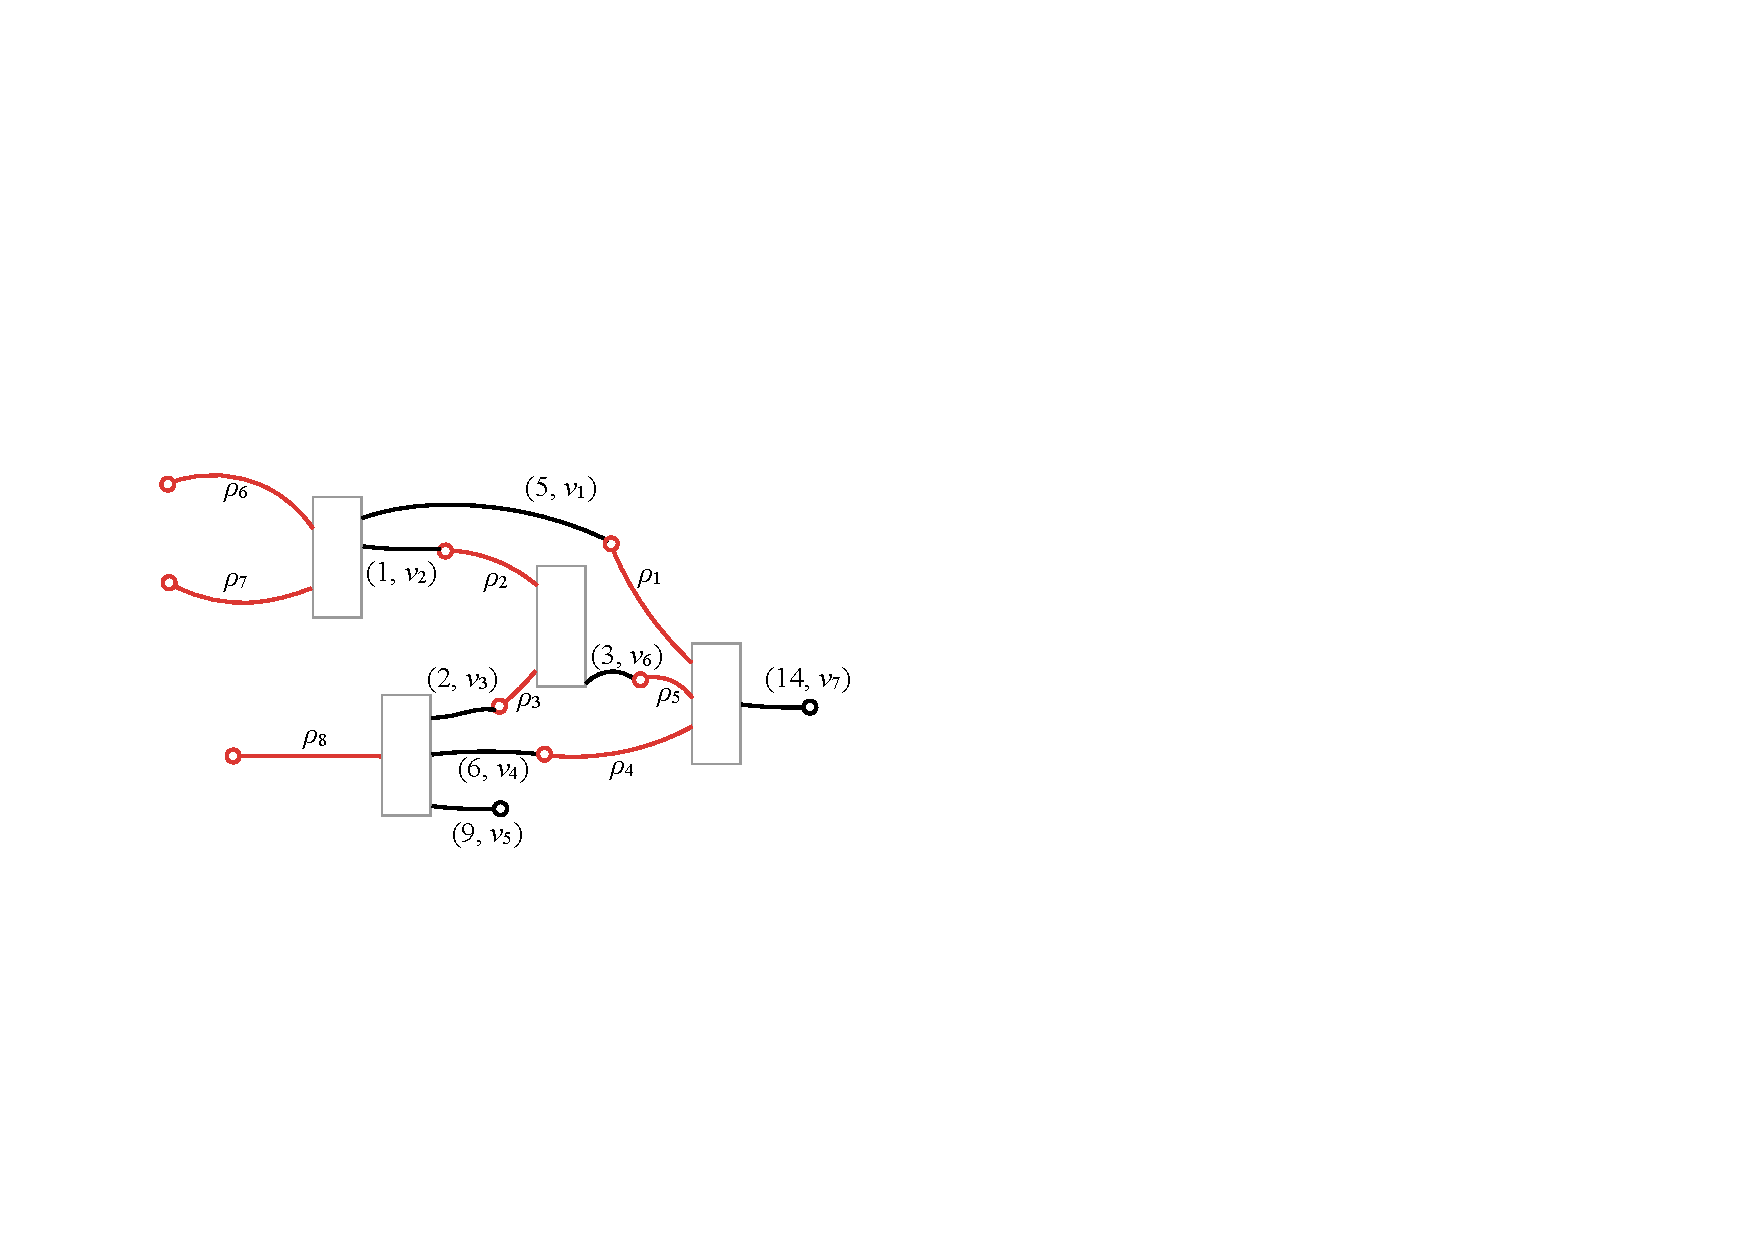
\includegraphics[width=\textwidth/2]{figures/utxo-graph.pdf}
 \caption{Example of a plain UTxO graph}
  \label{fig:utxo-graph}
\end{figure}

\subsection{Extended UTxO}
The basis for our fast isomorphic state channels is Bitcoin's UTxO ledger model~\cite{formal-model-of-bitcoin-transactions,Zahnentferner18-UTxO}. It arranges transactions in a directed acyclic graph structure, thus making the available parallelism explicit: 

\emph{Any two transactions that are not directly or indirectly dependent on each other can be processed independently.}

This arrangement results in graphs, such as the one in Figure~\ref{fig:utxo-graph},
where the boxes represent transactions with (red) inputs to the left and (black) outputs to the
right.

The set of dangling (unconnected) outputs are the \emph{unspent transaction outputs (UTxOs)} --- there are two of those in Figure~\ref{fig:utxo-graph}. 

\subsubsection{Notations}

In the rest of this document, we use of the following loosely specified functions and values: 
\begin{itemize}
   \item  $\mathbb{B} = \{0,1\}^k$ denotes a string of $k$ bits, eg. an arbitrary string of bytes, 
    \item $\mathbb{H} : \alphat \to \mathbb{B}$ denotes a \emph{hashing} function mapping arbitrary data to bytes, 
    \item $\mathsf{bits} : \alpha \to \mathbb{B}$ denotes a \emph{serialisation} function mapping arbitrary data to bytes,
    \item $k$, $k'$, $k_i$ denote \emph{verification keys},
\end{itemize}

\subsubsection{Definitions}

\begin{definition}[Values]

$\mathsf{Val}$ is a \emph{set} of \emph{tokens} represented as a tuple $(\mathsf{pid} \rightarrow \mathsf{tok} \rightarrow q)$ where
\begin{itemize}
    \item $\mathsf{pid} \in \{0,1\}^k$ is the \emph{Minting Policy identifier}, an arbitrary string of bytes corresponding to the \emph{hash} of a corresponding \emph{Minting Policy script},
    \item $\mathsf{tok} \in \{0,1\}^k$ is the \emph{Token name}, an arbitrary string of bytes,
    \item $q \in \mathbb{Z}$ is the quantity of this particular token.
\end{itemize}
Minting policy scripts are denoted $\mu$ and specific values are denoted $\mathsf{val}_{x}$ where $x$ identifies the output holding the value.
\end{definition}

\begin{definition}[Validator Script]
A validator script $\nu$ is a pure function whose type is:
\[
  \nu : (\delta : \txDataTy) \to (\rho : \txDataTy) \to (\mathsf{tx} : \txPendingTxTy)
  \to\txBoolTy,
\]
where: 
\begin{itemize}
    \item $\txDataTy$ is a universal data type, and we denote an empty value of type $\txDataTy$ by $\emptyset$,  
    \item $\delta$ is the \emph{datum} part of the output to which this particular script is locked (see Definition \ref{def:outputs}),
    \item $\rho$ is the \emph{redeemer} provided as part of the transaction being validated,
    \item $\txBoolTy = \{\bot, \top\},$
    \item $\txPendingTxTy$ is the \emph{validation context}.
\end{itemize}
\end{definition}

Validator scripts are called \emph{phase-2} scripts in the Alonzo Ledger specification (see \cite{alozon-spec} for a formal treatment of these). Informally, scripts are \emph{evaluated} by the ledger when it \emph{applies} a transaction to its current state to yield a new ledger state. Each validator script referenced by an output is passed its arguments drawn from the output it locks and the transaction context it is executed in. The transaction is valid if and only if all scripts evaluates to $\top.$

We denote by $V$ the set of all validator scripts.

\begin{definition}[Outputs]
An \emph{output} $o$ is a triple $\mathsf{Val} \times V \times \txDataTy$ 
For the purpose of this specification, each output \(o \in O\) is a triple of a value
$\txVal$, a validator script $\nu$, and a datum $\delta$.
\end{definition}


\begin{definition}[Inputs]
$$\txOutRef = (\mathsf{txId} \times \mathsf{outIx})$$
$$i \in I = (\txOutRef \times \rho)$$

Each input \(i\in I\) is a pair consisting of an \emph{output reference} $\txOutRef$ and a \emph{redeemer} $\rho$, where $\txOutRef$ consists of a transaction ID ($\mathsf{txId}$) and an index identifying an output in the transaction ($\mathsf{outIx}$).
\end{definition}

\begin{definition}[Validation Context]

$\txPendingTxTy$ provides validators with additional context pertaining to the transaction being validated. More specifically, it provides:
\[
  i = (\txOutRef, \rho)
\]
\[
 \txIpend \in \txIpendSet = (i, o)
\]
\[
 \txPendingTx \in \txPendingTxTy = (\txIpendSet \times O \times \txValForge \times r \times \txKeys) 
\]
such that $o$ is the output of the
consumed transaction referred to by $\txOutRef$.

In Figure~\ref{fig:utxo-graph}, we use pairs \((n, \nu)\) to indicate that a given output locks $n$ cryptocurrency with validator predicate $\nu$.
\end{definition}


\begin{definition}[Transactions]
$$
\tx = (I \times O \times \txValForge \times r \times \txKeys)
$$ 
comprising a set of
\emph{inputs} $I$, a list of \emph{outputs} $O$, values of
\emph{minted/burned tokens} $\txValForge$, a \emph{slot range}
\(r = (\txRmin, \txRmax)\), and a set of public keys $\txKeys$.

The slot range $r$ indicates the slots within which $\tx$ may be
confirmed and, finally, $\txKeys$ are the public keys under which
$\tx$ is signed.

In order to validate a transaction $\tx$ with input set $I$, for each
output $o = (\txVal,\nu,\delta)$ referenced by an
$i = (\txOutRef,\rho) \in I$, the corresponding validator $\nu$ is run
on the following inputs:
\(
  \nu(\txVal,\delta,\rho,\txPendingTx),
\)
where the validation context $\txPendingTx$ consists of $\tx$ and \emph{all} outputs
referenced by some $i \in I$ (not just $o$). Ultimately, $\tx$ is
valid if and only if all validators return $\true$.
\end{definition}

\vspace{5mm} The \emph{Extended UTxO Model (EUTxO)}~\cite{eutxo} preserves this structure, while adding support for more expressive smart contracts and, in particular, for multi-transaction state machines, which serve as the basis for the mainchain portion of the Hydra protocol. 

This additional expressiveness is achieved by two changes to the plain UTxO scheme outlined before: 

\begin{itemize}
\item Outputs carry, in addition to a cryptocurrency value $n$ and a validator $\nu$, now also a \emph{datum} $\delta$, which can, among other things, be used to maintain the state of long running smart contracts.
\item The validation context $\sigma$ is extended to contain the entire validated transaction $\txTx$ as well as the UTxOs consumed by the inputs of that transaction.
\end{itemize}

In this extended model, evaluation of the validator predicate implies checking \(\nu(\rho, \delta, \sigma) = \true\). Besides maintaining contract state in $\delta$, the fact that the validator can inspect the entire validated transaction $\txTx$ through $\sigma$ enables validators to enforce that contract invariants are maintained across entire chains of transactions.

Although formal results about EUTxO are rather recent, extended UTxO models already form the basis for the smart-contract platforms of existing blockchains --- in particular, Cardano~\cite{plutus-platform} and Ergo~\cite{ergo-platform}. Consequently, the Hydra head protocol as presented in this paper is of immediate practical relevance to these existing systems.

\subsection{User-defined tokens}

In addition to the basic EUTxO extension, we generalize the currency \emph{values} recorded on the ledger from integral numbers to \emph{generalized user-defined tokens}~\cite{eutxo-2}.

% \begin{definition}[Validator Validity]
%   Given a pending transaction $\txPendingTx$, the script-controlled
%   spending conditions are fulfilled iff the following holds, for
%   each \(\txIpend\in\txIpendSet\) with
%   \(\txIpend = ((\txOutRef, \rho), (\txVal, \nu, \delta))\)
%   \[
%     \nu(\txVal, \delta, \rho, \txPendingTx) = \top
%   \]
%   Note that the above ignores all inputs that spend pay-to-pubkey
%   outputs due to the required format for referenced outputs.
% \end{definition}

% Validators may make use of the following two helper functions:
% \(\txUTxO{\txIpendSet} = \{ o \mathbin| (i, o) \in \txIpendSet \}\)
% and
% %
% \begin{align*}
%   &\txValue{\txIpendSet}         & &= \txValue{\txUTxO{\txIpendSet}} \\
%   &\txValue{O}                   & &= \Sigma_{o \in O} \txValue{o} \\
%   &\txValue{\txVal, \kappa}      & &= \txVal \\
%   &\txValue{\txVal, \nu, \delta} & &= \txVal 
% \end{align*}

\subsection{State Machines}
%\label{sec:state_machines}
A convenient abstraction for EUTxO smart contracts spanning a sequence
of related transactions are state machines. Specifically, we adopt
\emph{constraint emitting machines (CEMs)}~\cite{eutxo}. These are
based on Mealy machines and consist of a set of states $\cemS$, a set
of inputs $\cemI$, a predicate \(\cemFinal : \cemS\to\txBoolTy\)
identifying final states, and a step relation
\(\cemStepRel{s}{i}{s'}{\cemTxCon}\), which takes a state $s$ on an
input $i$ to a successor state $s'$ under the requirements that the
constraints $\cemTxCon$ are satisfied.

We implement CEMs on a EUTxO ledger (the mainchain) by representing a sequence of CEM states as a sequence of transactions. Each of these transactions has got a \emph{state-machine input} $\cemIn$ and a \emph{state-machine output} $\cemOut$, where the latter is locked by a validator $\cemVal$, implementing the step relation. The only exceptions are the initial and final state, which have got no state-machine input and output, respectively.

\begin{figure}[t]
  \centering
  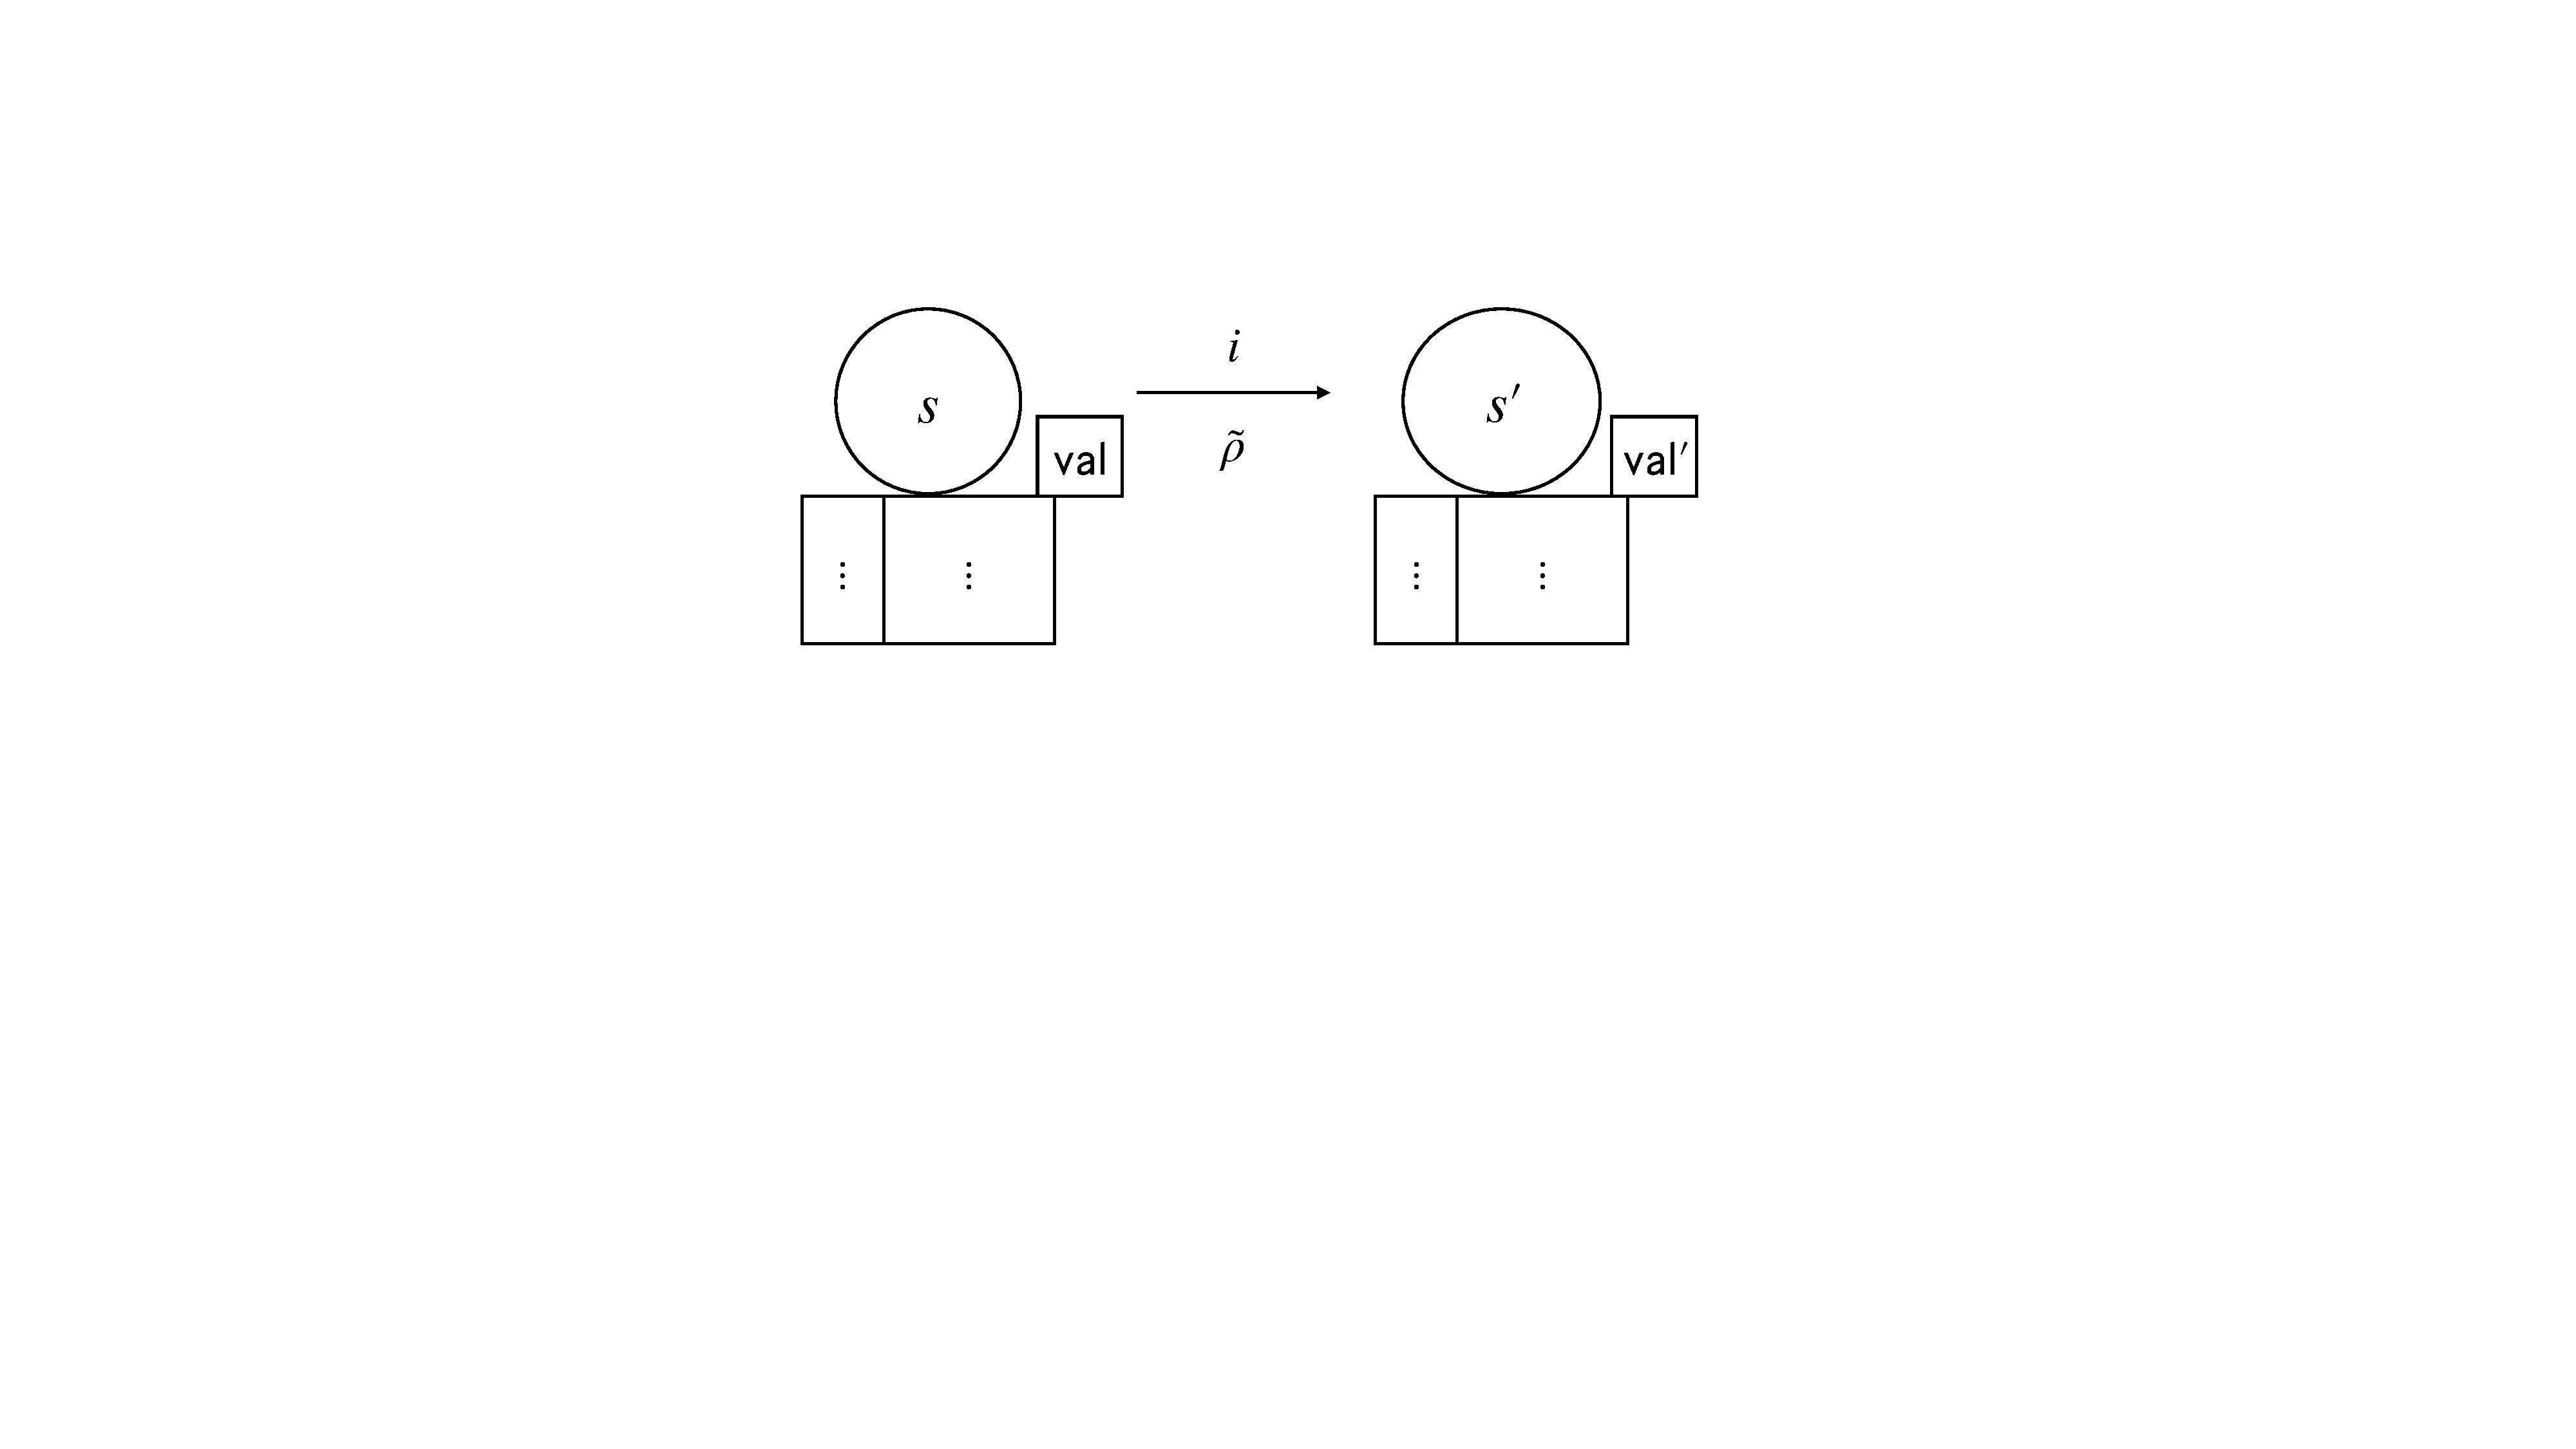
\includegraphics[scale=.2,width=\textwidth/2]{figures/state-transition_cropped.pdf}
  \caption{Transactions representing successive states in a CEM
    transition relation \(\cemStepRel{s}{i}{s'}{\cemTxCon}\).  Fields
    $\val$ and $\val'$ are the value fields of the state-machine
    outputs and $\tilde \rho$ is the additional data.}
  \label{fig:state-transition}
\end{figure}

More specifically, given two transactions $\tx$ and $\tx'$, they represent successive states under \(\cemStepRel{s}{i}{s'}{\cemTxCon}\) iff 

\begin{mitemize}
  \item state-machine output $\cemOut = (\txVal, \cemVal, s)$ of $\tx$
  is consumed by the state-machine input $\cemIn' = (\txOutRef, \rho)$
  of $\tx'$, whose redeemer is \(\rho = i\) (i.e., the redeemer
  provides the state-machine input) and
  \item either $\cemFinal(s') = \true$ and $tx'$ has no state-machine
  output, or $\cemOut' = (\txVal', \cemVal, s')$ and $\tx'$ meets all
  constraints imposed by $\cemTxCon$.
\end{mitemize}
Sometimes it is useful to have additional data $\tilde \rho$ provided
as part of the redeemer, i.e., $\rho = (i,\tilde \rho)$.

A state transition of the described type is represented by two connected
transactions as shown in Fig.~\ref{fig:state-transition}.  For
simplicity, state-machine inputs and outputs are not shown, with the
exception of the value fields $\txVal$ and $\txVal'$ of the state-machine output.


%%% Local Variables:
%%% mode: latex
%%% TeX-master: "main"
%%% End:
